\subsection{Vector Functions and Space Curves}

\begin{definition}[Vector function]
$\mathbf{r}(t) = \begin{pmatrix} x(t) \\ y(t) \\ z(t) \end{pmatrix}$
describes a position vector on a curve in 3D.
\end{definition}

\begin{center}
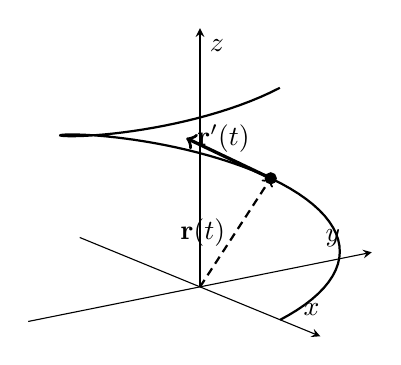
\begin{tikzpicture}
    \begin{axis}[
        view={55}{25}, width=9cm, height=7cm,
        xlabel=$x$, ylabel=$y$, zlabel=$z$,
        axis lines=center, ticks=none,
        xmin=-1.5, xmax=1.5, ymin=-1.5, ymax=1.5, zmin=0, zmax=7,
    ]
    % helix curve
    \addplot3[thick, domain=0:6.28, samples=80, samples y=0]
        ({cos(deg(x))},{sin(deg(x))},{x});
    % position vector r(t) at t=2
    \draw[->, thick, densely dashed] (axis cs:0,0,0)
        -- (axis cs:{cos(deg(2))},{sin(deg(2))},2)
        node[midway, left]{$\mathbf{r}(t)$};
    % tangent vector r'(t) at t=2
    \draw[->, very thick] (axis cs:{cos(deg(2))},{sin(deg(2))},2)
        -- (axis cs:{cos(deg(2))-0.7*sin(deg(2))},{sin(deg(2))+0.7*cos(deg(2))},2.7)
        node[right]{$\mathbf{r}'(t)$};
    % point
    \addplot3[only marks, mark=*, mark size=2pt]
        coordinates {({cos(deg(2))},{sin(deg(2))},2)};
    \end{axis}
\end{tikzpicture}
\end{center}

\begin{example}
$\mathbf{r}(t) = \begin{pmatrix} \dfrac{5+t^{2}}{5-t^{2}} \\[6pt] t\arctan t \\[6pt] \dfrac{5-e^{2t}}{t} \end{pmatrix}$

\[
    \lim_{t\to 0}\mathbf{r}(t)
    = \begin{pmatrix} 1 \\ 0 \\ \text{DNE} \end{pmatrix}
    = \text{DNE}
\]
\end{example}

$\mathbf{r}(t)$ is continuous $\;\Longleftrightarrow\;
\displaystyle\lim_{t\to a}\mathbf{r}(t) = \mathbf{r}(a)$. \;
Like single variable.

\begin{example}[Parametrize an intersection]
Cylinder $x^{2}+y^{2}=1$ \;\&\; paraboloid $z = x^{2}+y^{2}+x$.

\[
    \begin{cases} x^{2}+y^{2}=1 \\ z=x^{2}+y^{2}+x \end{cases}
    \;\Longrightarrow\; z = x+1
\]
Intersection lies on the plane $z=x+1$.
On the cylinder, choose $x=\cos t$, $y=\sin t$:
\[
    \mathbf{r}(t)
    = \begin{pmatrix} \cos t \\ \sin t \\ \cos t + 1 \end{pmatrix}
\]
\end{example}

\subsection{Derivatives and Integrals}

\subsubsection*{Derivatives}

\[
    \mathbf{r}'
    = \begin{pmatrix} x' \\[4pt] \vdots \end{pmatrix}
    = \lim_{h\to 0}\frac{\mathbf{r}(t+h)-\mathbf{r}(t)}{h}
\]

In the limit, $\dfrac{d\mathbf{r}}{dt}$ is tangent to $\mathbf{r}(t)$.

Speed: $v = \lVert\mathbf{r}'\rVert = \sqrt{x'^{2}+y'^{2}+z'^{2}}$

\begin{example}
$\mathbf{r}(t) = \begin{pmatrix} t \\ t^{2} \\ \cos t \end{pmatrix}$, \quad
$\mathbf{r}'(t) = \begin{pmatrix} 1 \\ 2t \\ -\sin t \end{pmatrix}$

$v(t) = \sqrt{1+4t^{2}+\sin^{2}t}$

Unit tangent vector:
$\mathbf{T}(t) = \dfrac{\mathbf{r}'}{\lVert\mathbf{r}'\rVert}
= \dfrac{1}{\sqrt{1+4t^{2}+\sin^{2}t}}
\begin{pmatrix} 1 \\ 2t \\ -\sin t \end{pmatrix}$
\end{example}

\begin{example}[Helix]
$\mathbf{r}(t) = \begin{pmatrix} \cos t \\ \sin t \\ t \end{pmatrix}$, \quad
$\mathbf{r}'(t) = \begin{pmatrix} -\sin t \\ \cos t \\ 1 \end{pmatrix}$

Speed: $v(t) = \lVert\mathbf{r}'\rVert = \sqrt{\sin^{2}t+\cos^{2}t+1} = \sqrt{2}$
\end{example}

\subsubsection*{Derivative Rules}

\begin{align*}
    \frac{d}{dt}(\mathbf{r}+\mathbf{s}) &= \mathbf{r}'+\mathbf{s}' &
    \frac{d}{dt}(\lambda\mathbf{r}) &= \lambda'\mathbf{r}+\lambda\mathbf{r}' \\[4pt]
    \frac{d}{dt}(\mathbf{r}\cdot\mathbf{s}) &= \mathbf{r}'\cdot\mathbf{s}+\mathbf{r}\cdot\mathbf{s}' &
    \frac{d}{dt}(\mathbf{r}\times\mathbf{s}) &= \mathbf{r}'\times\mathbf{s}+\mathbf{r}\times\mathbf{s}'
\end{align*}

\subsubsection*{Integration}

\[
    \int_{a}^{b}\mathbf{r}\dd{t}
    = \begin{pmatrix} \int_{a}^{b}x\dd{t} \\[4pt] \vdots \end{pmatrix}
\]

\begin{example}
\[
    \int_{0}^{1}\begin{pmatrix} t \\ e^{2t} \\ t^{2} \end{pmatrix}\dd{t}
    = \begin{pmatrix} \frac{1}{2}t^{2} \\[4pt] \frac{1}{2}e^{2t} \\[4pt] \frac{1}{3}t^{3} \end{pmatrix}\Bigg|_{0}^{1}
    = \begin{pmatrix} \frac{1}{2} \\[4pt] \frac{1}{2}(e^{2}-1) \\[4pt] \frac{1}{3} \end{pmatrix}
\]
\end{example}

\begin{example}[Angle between curves]
$\mathbf{r}(t) = \begin{pmatrix} t^{3} \\ t \\ t \end{pmatrix}$, \;
$\mathbf{s}(t) = \begin{pmatrix} t \\ \sin t \\ t \end{pmatrix}$.
Find the angle of intersection at $(0,0,0)$.

$\mathbf{r}' = \begin{pmatrix} 3t^{2} \\ 1 \\ 1 \end{pmatrix}$, \;
$\mathbf{s}' = \begin{pmatrix} 1 \\ \cos t \\ 1 \end{pmatrix}$

At $t=0$: \;
$\mathbf{r}'\cdot\mathbf{s}' = \lVert\mathbf{r}'\rVert\,\lVert\mathbf{s}'\rVert\cos\theta$
\[
    \cos\theta = \frac{2}{\sqrt{2}\cdot\sqrt{3}} = \sqrt{\tfrac{2}{3}}
    \qquad
    \theta = \cos^{-1}\!\sqrt{\tfrac{2}{3}} \approx 35^{\circ}
\]
\end{example}

\subsection{Arc Length and Curvature}

\begin{definition}[Arc length]
\[
    L = \int_{t_{0}}^{t_{1}}\lVert\mathbf{r}'(t)\rVert\dd{t}
    = \int_{t_{0}}^{t_{1}}v(t)\dd{t}
\]
\end{definition}

\begin{example}[Helix arc length]
From $t=0$ to $t=2\pi$:
\[
    \int_{0}^{2\pi}v(t)\dd{t}
    = \int_{0}^{2\pi}\sqrt{2}\dd{t}
    = 2\pi\sqrt{2}
\]
\end{example}

\begin{definition}[Curvature]
On a point of $\mathbf{r}(t)$, imagine force $\mathbf{F}=\mathbf{r}''$.
Curvature measures this only when speed $=1$.
\end{definition}

\begin{example}[Helix with unit speed]
$\mathbf{r}(t)
= \begin{pmatrix} \sin(t/\!\sqrt{2}) \\ \cos(t/\!\sqrt{2}) \\ t/\!\sqrt{2} \end{pmatrix}$, \quad
$\mathbf{r}'
= \dfrac{1}{\sqrt{2}}
\begin{pmatrix} \cos(t/\!\sqrt{2}) \\ -\sin(t/\!\sqrt{2}) \\ 1 \end{pmatrix}$
$\;\Longrightarrow\;$ speed $= 1$

\[
    \kappa = \lVert\mathbf{r}''\rVert
    = \left\lVert \frac{1}{2}
    \begin{pmatrix} -\sin(t/\!\sqrt{2}) \\ -\cos(t/\!\sqrt{2}) \\ 0 \end{pmatrix}
    \right\rVert
    = \frac{1}{2}
\]
\end{example}

\subsubsection*{Curvature when speed $\neq 1$}

Reparametrize by arc length: $\kappa(t) = \kappa(t(s))$ so that speed $= 1$ w.r.t.\ $s$.

\[
    \frac{d\mathbf{r}}{ds}
    = \frac{dt}{ds}\,\frac{d\mathbf{r}}{dt}
    \;\Longrightarrow\;
    \frac{ds}{dt} = \lVert\mathbf{r}'(t)\rVert = v(t)
\]

Since $\mathbf{r}'(t) = v(t)\,\mathbf{T}(t)$ where $\mathbf{T}$ is the unit tangent:

\[
    \kappa
    = \lVert\mathbf{r}''(s)\rVert
    = \frac{d}{ds}\!\left(\frac{\mathbf{r}'(t)}{v(t)}\right)
    = \frac{\lVert\mathbf{T}'(t)\rVert}{v(t)}
    = \boxed{\frac{\lVert\mathbf{r}'\times\mathbf{r}''\rVert}{v(t)^{3}}}
\]

\begin{example}[Curvature of $y=f(x)$]
Let $\mathbf{r}(t) = \begin{pmatrix} t \\ f(t) \\ 0 \end{pmatrix}$.
Then
\[
    \kappa(t)
    = \frac{\lVert\mathbf{r}'\times\mathbf{r}''\rVert}{v(t)^{3}}
    = \frac{\lvert f''(t)\rvert}{\bigl(1+f'(t)^{2}\bigr)^{3/2}}
\]
\end{example}

\begin{example}[Motion in space]
$t$: time, \; $\mathbf{r}(t)$: position, \;
$\mathbf{v}(t)=\mathbf{r}'(t)$: velocity, \;
$\mathbf{a}(t)=\mathbf{v}'(t)$: acceleration

Newton's second law: $\mathbf{F}=m\mathbf{a}$ \; (differential equation).

Gravity: $\mathbf{F}=-mg\,\hat{\mathbf{k}}$ where $\hat{\mathbf{k}}$ is the unit vector in $z$.
\[
    -mg\,\hat{\mathbf{k}} = m\,\mathbf{r}''(t)
    \;\Longrightarrow\;
    \mathbf{r}'' = -g\,\hat{\mathbf{k}}
\]
Integrating:
\begin{align*}
    \mathbf{r}' &= -gt\,\hat{\mathbf{k}} + \mathbf{C}_{0} \\
    \mathbf{r}  &= -\tfrac{1}{2}g t^{2}\,\hat{\mathbf{k}}
                   + \mathbf{C}_{0}\,t + \mathbf{C}_{1}
\end{align*}
\end{example}
